\documentclass[a4paper, 11pt]{scrreprt}
\usepackage[ngerman]{babel}
\usepackage{csquotes} % it necessary for using babel
\usepackage{float} % for positioning images
\usepackage{graphicx} % inclusion of graphics & pdfs
% \usepackage[ansinew]{inputenc} % um Umlaute direkt einbinden zu können
\usepackage{enumitem}
\usepackage{hyperref} % so links to other chapters etc. in doc
\usepackage{xcolor} % more colors etc.

\usepackage{listings} % for code

\usepackage[a4paper, left=3cm, right=3cm, top=2cm]{geometry} % Randbreite 3cm links und rechts
\usepackage[onehalfspacing]{setspace} % Zeilenabstand 1,5x
%\usepackage{setspace}
%\spacing{1,2381}

\usepackage{helvet} % use instead of arial because it is basically the same
\renewcommand{\familydefault}{\sfdefault} % set helvet as default family

\usepackage[
    style=authoryear,
    doi=false,
    isbn=false,
    url=false,
    eprint=false,
    backend=biber]{biblatex} %citation

\DeclareFieldFormat{postnote}{\mknormrange{#1}}
\DeclareFieldFormat{volcitepages}{\mknormrange{#1}}
\DeclareFieldFormat{multipostnote}{\mknormrange{#1}}

\usepackage[
    activate={true,nocompatibility},
    final,tracking=true,
    kerning=true,
    spacing=true,
    factor=1100,
    stretch=10,
    shrink=10]{microtype}

\setcounter{tocdepth}{3}
\setcounter{secnumdepth}{3}

\counterwithout{figure}{chapter} % figure numbering

\usepackage{scrhack}

%\setlength{\marginparwidth}{2cm} % added because of todo notes
%\usepackage[textsize=scriptsize, color=blue!40!white, colorinlistoftodos]{todonotes}
% thesis information
\newcommand*{\getUniversity}{Hochschule Konstanz Technik, Wirtschaft und Gestaltung}
\newcommand*{\getFaculty}{Fakultät Informatik}
\newcommand*{\getDoctype}{Bachelor Thesis in der Wirtschaftsinformatik, \ldots}
\newcommand*{\getSupervisor}{Lisa-Maria Reutlinger}
\newcommand*{\getAdvisor}{Prof. Dr. Markus Eiglsperger} % oder anders herum?
\newcommand*{\getSubmissionLocation}{Konstanz am Bodensee}

\title{Wie kann durch technikgestütze Kommunikation die Phase der Qualitätssicherung eines agilen Teams minimiert werden?}
\author{Sonja Jolanda Klein}
\date{15.06.2023}

\addbibresource{quellen/citavi.bib}
\begin{document}
%\listoftodos[ToDos]

\pagenumbering{roman}
\input{seiten/cover}
\tableofcontents
\addcontentsline{toc}{chapter}{Abbildungsverzeichnis}
\listoffigures
\newpage
\pagenumbering{arabic}
\chapter{Das Problem}
Das Open Pouring Problem wird formal wie folgt beschrieben: Es seien drei Krüge mit unterschiedlichen Kapazitäten gegeben, die jeweils eine ganzzahlige Menge an Wasser enthalten. 
In jedem Schritt darf eine Wassermenge, die höchstens der aktuellen Wassermenge eines Kruges entspricht, von einem Krug in einen anderen gegossen werden. Das Ziel ist es, durch eine Reihe solcher Schritte einen der Krüge vollständig zu leeren, das heißt, seine Wassermenge auf null zu reduzieren.

\begin{figure}[H]
    \centering
    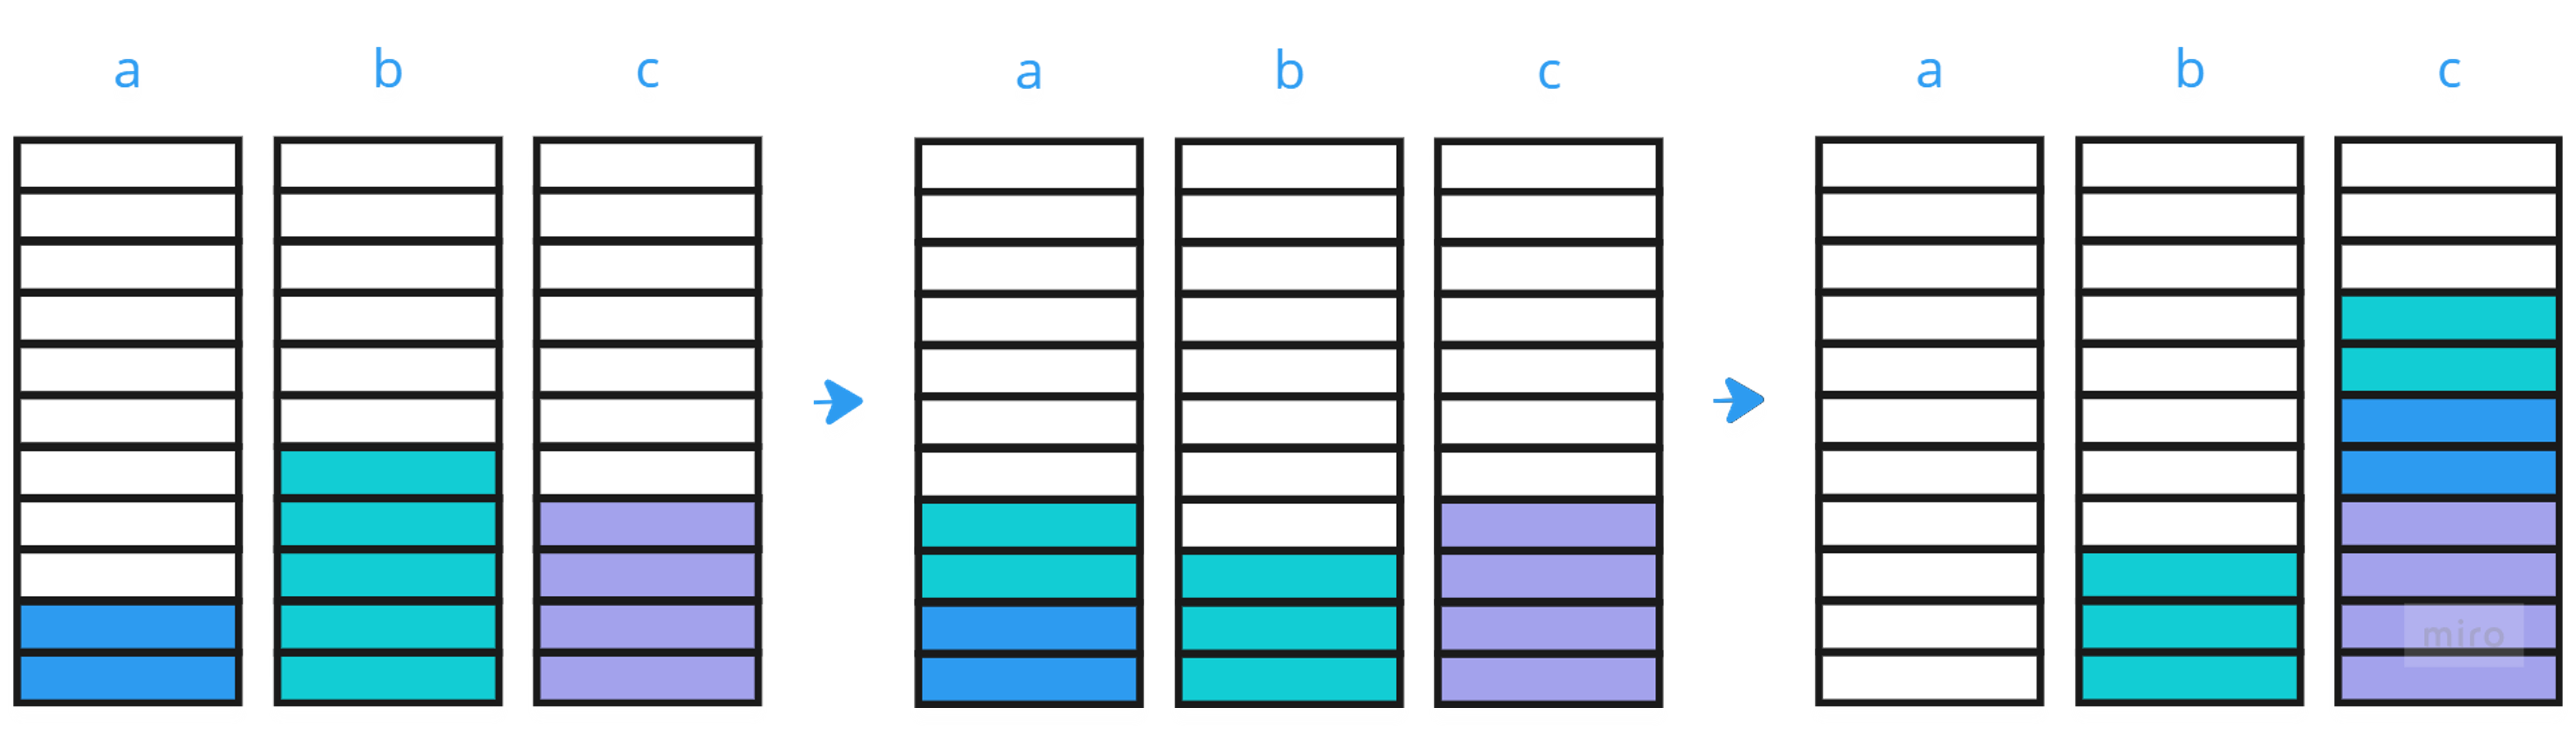
\includegraphics[page=1, width=1\textwidth]{./bilder/Pouring_Problem_1.png} 
    \caption{Pouring Problem: ein einfaches Beispiel mit zwei, fünf und 4 Litern in der Anfangskonfiguration} 
    \label{fig:pouring_problem_die_hard}
\end{figure}

Die mathematische Modellierung des Problems erfolgt durch die Definition einer Konfiguration als Tripel $(a, b, c)$, wobei $a$, $b$ und $c$ die Wassermengen in den drei Krügen darstellen. Das Problem besteht darin, eine Sequenz von Operationen zu finden, die eine Ausgangskonfiguration $(a, b, c)$ in eine Endkonfiguration $(a', b', 0)$ überführt. Die Herausforderung liegt darin, die minimale Anzahl der erforderlichen Schritte zu bestimmen, die in allen möglichen Konfigurationen benötigt werden.
\chapter{Lösungsansatz} 
Das hier vorgestellte Paper \autocite{Frei.2020} stellt einen algorithmischen Ansatz vor, der das Problem für eine gegebene Konfiguration löst. Der Algorithmus arbeitet in sogenannten \emph{'Runden'}, wobei jede Runde aus mehreren Schritten besteht. Der Ausgangspunkt jeder Runde ist die Sortierung der Wassermengen in den Krügen, gefolgt von der Berechnung bestimmter Parameter, die die nächsten Schritte bestimmen. Es werden zwei Hauptfälle unterschieden, die je nach Verhältnis der Wassermengen in den Krügen unterschiedlich behandelt werden.

\section{Der Ablauf innerhalb einer Runde} \label{runden} 
Eine Runde startet mit einer Anfangskonfiguration $(a, b, c)$ mit $0 < a\leq b \le c$ und endet mit einer Konfiguration $(a', b', c')$ mit $a' \leq a/2$. Wenn eine der drei Zahlen nach einer Runde 0 ist, ist das Ziel erreicht. \\
Eine Runde ist immer folgendermaßen aufgebaut:

\begin{itemize}
    \item Sortieren der Krüge, sodass $a \leq b \leq c$
    \item die Hilfswerte $r$, $p$, $q$ berechnen
    \item Fall 1 oder Fall 2 ausführen je nachdem ob $b-pa \leq a/2$ gilt.
    \item Prüfen ob wir unser Ziel erreicht haben
\end{itemize}  

\section{Berechnung der Hilfswerte r, p und q} \label{helper}
Die Hilfswerte werden folgendermaßen berechnet:
    %$r \coloneq b/a$, 
    %$p \coloneq \lfloor r \rfloor $ und
    %$q \coloneq \lceil r \rceil $.
Dabei können wir etwas festellen. Es gilt: $0 \leq b-pa < a $ und $ 0 \leq qa - b < a $. 
Das impliziert dass $min(b-pa, qa-b) \leq a/2$, da $(b-pa)+(qa-b)=(q-p)a \leq a$. 
Außerdem betrachten wir die kleinsten binären Repräsentationen von $p$ und $q$: $p_k...p_0$ und $q_\ell...q_0$. Diese werden im Verlauf von Fall 1 und Fall 2 relevant.
\section{Fall 1} \label{case-1}
Aus den Hilfswerten prüfen wir die Bedingung $b-pa \leq a/2$. Wenn diese eintritt, dann führen wie Fall 1 aus, wenn nicht, dann gilt $qa-b < a/2$ und wir führen Fall 2 aus. \\
In Fall 1 führen wir $k+1$ Schritte für $i=0, ..., k$ aus, die immer das verdoppeln werden was anfänglich $a$ war. Dazu muss erst $a$, dann $2a$ und allgemein $2^ia$ von einer der anderen Nummern abgezogen werden. 
Wir ziehen den benötigten Betrag 
\begin{itemize}
    \item von der zweiten Nummer ab (anfänglich $b$), wenn $p_i = 1$ und
    \item von der dritten Nummer ab (anfänglich $c$), wenn $p_i = 0$.
\end{itemize}

Nach der Ausführung dieser $k+1$ Schritte, sind die zweite und die dritte Nummer $b- \sum_{i=0}^{k} p_i2^ia = b-pa \leq a/2$ bzw. $c- \sum_{i=0}^{k} (1-p_i)2^ia$. Die zweite Nummer $b-pa \leq a/2$ gleicht der Bedingung, die wir geprüft haben um uns für Fall 1 zu entscheiden.

\section{Fall 2} \label{case-2}
% TODO: die ander Bedingung die dann auch erfüllt ist???
Wird die Bedingung $b-pa \leq a/2$ nicht erfüllt, dann führen wie Fall 2 aus. 
In Fall 2 gilt $qa-b < a/2$ und wir führen $\ell$ Schritte für $i=0, ..., \ell-1$ (und anschließend noch einen $(\ell +1)$-ten Schritt) aus, die immer das verdoppeln werden was anfänglich $a$ war. \\
Dazu muss wie in Fall 1 erst $a$, dann $2a$ und allgemein $2^ia$ von einer der anderen Nummern abgezogen werden. 
Anders als in Fall 1 jedoch ziehen wir den benötigten Betrag 
\begin{itemize}
    \item von der zweiten Nummer ab (anfänglich $b$), wenn $q_i = 1$ und
    \item von der dritten Nummer ab (anfänglich $c$), wenn $q_i = 0$.
\end{itemize}

Nach der Ausführung dieser $\ell$ Schritte, ist die erste Nummer $2^\ell a$, die zweite $b- \sum_{i=0}^{\ell-1} q_i2^ia = b-(q-2^\ell)a$ und die dritte Nummer $c- \sum_{i=0}^{\ell-1} (1-q^i)2^ia$. \\
Anschließend führen wir noch einen $(\ell +1)$-ten Schritt aus. Dieser macht aus $a = 2^\ell a- (b-qa+2^\ell a) = (-b+qa)$. \\
Die Runde endet und die erste Numer ist nun genau $(-b+qa) < a/2$. Sie gleicht der Bedingung, die wir geprüft haben um uns für Fall 2 zu entscheiden.
\chapter{Ein eigenes Beispiel} 
Um den Algorithmus besser verstehen zu können betrachten wir ihn an einem selbst gewählten Beispiel. Zur besseren Übersicht ist der Ablauf auch in Tabelle \ref{table:example} dargestellt. \\
Wir betrachten eine Konfiguration $(9, 8, 6)$. Der erste Schritt ist das Sortieren und erhalten $(6, 8, 9)$. \\
Als nächstes berechnen wir die Hilfswerte: $r=b/a=8/6_{10}$, $p=\lfloor r \rfloor = 1_{10}$ und $q=\lceil r \rceil = 2_{10}$. Daraus ergeben sich $p = 1_{2}$ und $q = 10_{2}$. \\
Als nächstes prüfen wir die Bedingung $b-pa \leq a/2$ und entscheiden aufgrund dessen, ob wir den Fall 1 oder Fall 2 betrachten. In diesem Fall ist die Bedingung erfüllt, also betrachten wir Fall 1. \\
In Fall 1 führen wir $k+1$ Schritte aus. Da $p= 1_{2}$ und $p_k...p_0$ führen wir also nur einen Schritt, Schritt 0, aus. In diesem Schritt verdoppeln wir was anfänglich a war, also $a'=2*a=2*6=12$. Dazu müssen wir diese 6 Liter aus einem der beiden anderen Krüge holen und da $p_0=1$ ist, holen wir laut der Regeln in Fall 1 die 6 Liter aus Krug b. Die neue Konfiguration ist also $(12, 2, 9)$. Damit haben wir die erste Runde abgeschlossen. Wir prüfen nun ob einer der drei Krüge nun leer ist. Da dies nicht der Fall ist beginnen wir mit Runde zwei.\\

In der zweiten Runde beginnen wir wieder mit Sortieren und erhalten $(2, 9, 12)$. Nun berechnen wir wieder die Hilfswerte: $r=b/a=9/2_{10}$, $p=\lfloor r \rfloor = 4_{10}$ und $q=\lceil r \rceil = 5_{10}$. Daraus ergeben sich $p = 100_{2}$ und $q = 101_{2}$. \\
Die Bedingung $b-pa \leq a/2$ ist dieses mal wieder erfüllt und wir betrachten wieder Fall 1. Dieses Mal haben wir jedoch $p=100_{2}$ und führen also drei Schritte aus. In Schritt 0 verdoppeln wir wieder a ($a'=2*a=2*2=4$) und holen die 2 Liter aus Krug c, da $p_0=0$. Wir erhalten $(4, 9, 10)$. In Schritt 1 verdoppeln wir wieder a ($a''=2*a'=2*4=8$) und holen die 4 Liter aus Krug c', da $p_1=0$. Wir erhalten $(8, 9, 6)$. In Schritt 2 verdoppeln wir wieder a ($a'''=2*a''=2*8=16$) und holen die 8 Liter aus Krug b'', da $p_2=1$. Wir erhalten $(16, 1, 6)$. Damit haben wir die zweite Runde abgeschlossen. Auch dieses Mal prüfen wir ob wir unser Ziel erreicht haben, aber noch keiner der drei Krüge ist leer, also brauchen wir noch eine weitere Runde.\\

In der dritten Runde erhalten wir nach dem Sortieren $(1, 6, 16)$. Die Hilfswerte sind $r=b/a=6/1_{10}$, $p=\lfloor r \rfloor = 6_{10}$ und $q=\lceil r \rceil = 6_{10}$. Daraus ergeben sich $p = 110_{2}$ und $q = 110_{2}$. \\
Dieses Mal ist die Bedingung $b-pa \leq a/2$ nicht erfüllt, also betrachten wir Fall 2. In Fall 2 führen wir zunächst $\ell$ Schritte aus und fügen am Schluss noch einen Schritt $\ell +1$ hinzu. \\
Auch hier verdoppeln wir a, sodass $a'=2*a=2$. Da wir uns dieses Mal in Fall 2 befinden, betrachten wir um zu entscheiden aus welchem Krug wir den Liter schütten nun $q$ und nicht mehr $p$. Da $q_0=0$ ist, holen wir den Liter aus Krug c und erhalten $(2, 6, 15)$. In Schritt 1 verdoppeln wir wieder a, sodass $a''=2*a'=4$. Da $q_1=1$ holen wir den Liter aus Krug b und erhalten $(4, 4, 15)$. Anschließend führen wir noch einen ($\ell+1$)-ten Schritt aus. Wir rechnen $a = 2^\ell a- (b-qa+2^\ell a) = (-b+qa)$, also $a'''=(-6+6*1)=0$ und erhalten $(8,0,15)$. %Todo das noch mal nach schauen was da jetzt genau war??
Damit sind wir fertig mit unserer dritten Runde. Da nun einer der Krüge leer ist, haben wir unser Ziel erreicht.\\

\begin{center}
	\begin{tabular}{ll}     
		ROUND 1: (9, 8, 6)                                                       \\
		\noindent\hspace*{12mm} 	SORTING:               (6, 8, 9)             \\ 
		\noindent\hspace*{12mm} 	HELPER: $p:1_{10}$ ($1_{2}$), $q:2_{10}$ ($10_{2}$)     \\
		\noindent\hspace*{12mm} 	CASE 1 (k=1):    				             \\
		\noindent\hspace*{22mm}			Step 0: $p_i = 1 \rightarrow (12, 2, 9)$    \\
		ROUND 2: (12, 2, 9)                                                      \\      
		\noindent\hspace*{12mm} 	SORTING... (2, 9, 12)                        \\
		\noindent\hspace*{12mm} 	HELPER: $p:4_{10}$ ($100_{2}$), $q:5_{10}$ ($101_{2}$   \\
		\noindent\hspace*{12mm} 	CASE 1 (k=3):                                \\
		\noindent\hspace*{22mm}			Step 0: $p_i = 0 \rightarrow (4, 9, 10)$    \\
		\noindent\hspace*{22mm}			Step 1: $p_i = 0 \rightarrow (8, 9, 6)$     \\
		\noindent\hspace*{22mm}			Step 2: $p_i = 1 \rightarrow (16, 1, 6)$    \\
		ROUND 3: (16, 1, 6)                                                      \\
		\noindent\hspace*{12mm} 	SORTING... (1, 6, 16)                        \\
		\noindent\hspace*{12mm} 	HELPER: $p:6_{10}$ ($110_{2}$), $q:6_{10}$ ($110_{2}$)  \\
		\noindent\hspace*{12mm} 	CASE 1 (k=3):                                \\
		\noindent\hspace*{22mm}			Step 0: $p_i = 0 \rightarrow (2, 6, 15)$    \\
		\noindent\hspace*{22mm}			Step 1: $p_i = 1 \rightarrow (4, 4, 15)$    \\
		\noindent\hspace*{22mm}			Step 2: $p_i = 1 \rightarrow (8, 0, 15)$    \\
		DONE in 3 rounds and 7 steps!                                            \\
	\end{tabular} \\
	\captionof{table}{Der Algorithmus benötigt 3 Runden und 7 Schritte um die Konfiguration $(9, 8, 6)$ in die Konfiguration $(8, 0, 15)$ zu überführen.}
	\label{table:example}
\end{center}

\chapter{Obere Schranke und Beweis für die Gültigkeit des Algorithmus} 
\textit{\textbf{Theorem 1:} Die optimale Anzahl von Schritten zur Lösung einer Instanz mit einer Gesamtliteranzahl von $n$ ist begrenzt durch $N(n) \leq (log(n))^2$.} \\

Im folgenden Abschnitt beweisen wir dass unser Algorithmus nur gültige Konfigurationen erreicht und erläutern die obere Schranke des Algorithmus. Dafür schauen wir uns die Schritte an, in welchen der Algorithmus die Konfigurationen verändert. Zuerst betrachten wir dabei Fall 1 genauer. \\
Wir müssen beweisen dass sowohl $b$ als auch $c$ aus der Anfangskonfiguration nach dem Umschütten groß genug sind um niemals negativ zu werden und so alle Schritte dieser Runde als gültig zu erklären. Für $b$ können wir einfach unsere Beobachtung $b-pa>=0$ nutzen (zur Erinnerung: $p=\lfloor b/a \rfloor$). 
Für $c$ haben wir $c-\sum_{i=0}^{k} (1-p_i) 2^i a = c-\sum_{i=0}^{k-1} (1-p_i) 2^i a = c-(\sum_{i=0}^{k-1} (2^i) - \sum_{i=0}^{k-1} (p_i 2^i))a \geq c-2^k a \geq 0$, bei der die letzte Ungleichheit aus $k=\lfloor log(p)\rfloor$ und $a \leq c$ resultiert. 
Wir schließen daraus, dass diese Runde machbar ist und zu einem Tripel führt, dessen kleinste Zahl höchstens $b-pa \leq a/2$  ist, wie gefordert. Die Anzahl der Schritte dieser Runde ist genau $k+1 = \lfloor log(p)\rfloor +1\leq \lfloor log(q)\rfloor +1$. \\

Als nächstes betrachten wir auch Fall 2 etwas genauer. Auch hier müssen wir beweisen dass diese $\ell$ Schritte tatsächlich möglich sind indem wir zeigen dass $b$ und $c$ groß genug sind. Dies ist der Fall, da wir auf der einen Seite $q \leq p+1$ haben und dadurch $b-(q-2^\ell)a \geq b-(q-2^0)a \geq b-pa \geq 0$ gilt, 
und auf der anderen Seite $c - \sum_{i=0}^{\ell -1} (1-q_i)2^ia \geq c-\sum_{i=0}^{\ell -1} (2^ia) = b-(2^\ell-1)a \geq b-(q-1)a \geq b-pa \geq 0$. Der letzte Schritt ist möglich, da $2^\ell a-(b-qa+2^\ell a)=qa-b \geq 0$.
Auch diese Runde ist machbar und endet mit genau $\ell+1=\lfloor log(q)\rfloor+1$ Schritten. Die erste Nummer des Tripels ist nun genau $qa-b<a/2$. \\

Wir haben gezeigt, wie man in beiden Fällen eine gültige Runde ausführt mit max $\lfloor log(q)\rfloor +1\leq \lfloor log(n/1)\rfloor +1$ Schritten, die mit einem Tripel $(a', b', c')$ endet, dessen kleinste Nummer maximal $a'\leq a/2$ ist. \\
Wie jede Konfiguration in aufsteigender Reihenfolge erfüllt die Anfangskonfiguration die Bedingungen $a \leq n/3$. Deshalb ist sichergestellt dass wir nach maximal $log(n-1)$ Runden eine Konfiguration erreichen, dessen kleinste Nummer maximal $n/3 * 2^{1-log(n)}=2/3 \approx 0$ ist. \\
Es reicht also aus, diesen gesamten Prozess für höchstens $\lfloor log(q)\rfloor -1$ Runden zu iterieren, und am Ende erhalten wir eine endgültige Konfiguration, deren kleinste Zahl $0$ ist. Die Gesamtanzahl der Schritte über alle Runden ist höchstens $(log(n)-1)*(log(n)+1) \leq (log(n))^2$. 
%\chapter{Untere Schranke} 
\textit{\textbf{Theorem 2:} Anzahl der Schritte zur Lösung eines Worst-Case-Falls mit einer Gesamtliterzahl von n ist mindestens $\lceil log ((n+1)/5) \rceil = \Omega (log(n))$} \\

Bisher haben wir nur die obere Schranke des Algorithmus betrachtet. In diesem Kapitel werden wir uns nun mit der unteren Schranke beschäftigen. \\

Sei $t:=n/3$ und $(a,b,c)$ je nach Rest von $mod 3$: 
\begin{equation}
    (a, b, c) = \begin{cases}
      (t-1, t, t+1) & \text{für } t-\lfloor t\rfloor = 0, \text{i.e.,} n \equiv 0 (mod (3))\\
      (t-(4/3), t-(1/3), t+(5/3)) & \text{für } t-\lfloor t\rfloor = 1/3, \text{i.e.,} n \equiv 1 (mod (3))\\
      (t-(5/3), t+(1/3), t+(4/3)) & \text{für } t-\lfloor t\rfloor = 2/3, \text{i.e.,} n \equiv 2 (mod (3))
    \end{cases}
 \end{equation}
Allgemein: $(t+d_1, t+d_2, t+d_3)$ mit $d_1<d_2<d_3$. \\

Dies können wir verallgemeinern zu einer Konfiguration nach $i$ Schritten. Nach 1 Schritt haben wir entweder $(2t+2d_1, d_2-d_1,t+d_3)$ oder $(2t+2d_1, t+d_2, d_3-d_1)$ oder $(t+d_1, 2t+2d_2,d_3-d_2)=(x_1, t+y_1, 2t+z_1)$.
Allgemein haben wir nach i Schritten: $(x_i, t+y_i, 2t+z_i)$. Daraus extrahieren wir die Werte $u$, $v$, $w$ und überlegen uns was dafür gilt. \\ 
Seien ${u_i, v_i, w_i }={|x_i |, |y_i |, |z_i |}$ und $u_i\leq v_i\leq w_i$. 
Für $i=1$ können wir direkt überprüfen dass $w_i\leq 5/3*2$ und $v_i\leq 5/3*2 -1/3$ ist. Allgemein gilt $w_i \leq 2w_{i-1}$ und $v_i\leq v_{i-1}+w_{i-1}$. Durch Induktion erhalten wir $u_i\leq v_i\leq w_i\leq 5/3*2^i$ und $v_i\leq 5/3*2^i  -1/3$ $\Rightarrow v_i+w_i\leq 5/3*2^(i+1) -1/3$. \\

Solange $v_i+w_i<t$ ist, können keine zwei der drei Zahlen die Summe $t$ ergeben, so dass $a, b, c$ nicht gleich sein können. Der einzige Weg zu einer Konfiguration, die eine $0$ enthält, führt jedoch über eine Konfiguration mit zwei gleichen Zahlen. Somit ist $v_i+w_i \geq t=n/3$ eine notwendige Bedingung für $(x_i, t+y_i, 2t+z_i)$, die Konfiguration nach Schritt $i$, die zwei gleiche Zahlen enthält. \\ 

Unsere Bedingung ist nicht erfüllt, solange diese beiden äquivalenten Ungleichungen wahr bleiben: $5/3*2^{i+1} -1/3<n/3  \Leftrightarrow i+1<log((n+1)/5)$. \\
Folglich muss jede Schrittzahl $k$, die uns eine Chance bietet, zwei gleiche Zahlen zu erhalten, $k+1\geq log(((n+1))/5)$ erfüllen. $\Rightarrow k\geq \lceil log((n+1)/5)  \rceil-1$. \\
Erst nach mindestens $k$ Schritten könnten zwei gleiche Zahlen in unserer Konfiguration auftauchen. Ein zusätzlicher Schritt mit diesen beiden Zahlen ist dann erforderlich, um eine Null zu erzeugen. Daher ist die Mindestanzahl der Schritte mindestens $\lceil log(((n+1))/5) \rceil= \Omega (log(n))$.
\chapter{Experimentelle Ergebnisse}
% Präsens und Präteritum
...
\chapter{Fazit}
% Präsens und Präteritum
???


\chapter*{Literaturverzeichnis}
\addcontentsline{toc}{chapter}{Literaturverzeichnis}
\printbibliography[heading=none]
\end{document}